\clearpage
\section{Scattering length density calculator}
\label{sec:SLDcalculator}

The \texttt{SLD calculator} is using thermal neutron cross-sections
only to calculate neutron scattering length density. For x-rays the
energy dependent scattering coefficients $f'$ and $f''$ are derived
using the theoretical approximation developed by Cromer and
Liberman. This theory gives accurate values far from an absorption
edge but does not account for the effects of neighboring atoms,
which can be very substantial near an absorption edge. Before
conducting an anomalous scattering experiment close to an absorption
edge it is therefore advisable to determine the actual scattering
behavior of the sample. The x-ray data have been taken from
\url{http://skuld.bmsc.washington.edu/scatter/AS_periodic.html} and
those for neutrons from
\url{http://www.ncnr.nist.gov/resources/n-lengths/list.html}.
\begin{figure}[htb]
\begin{center}
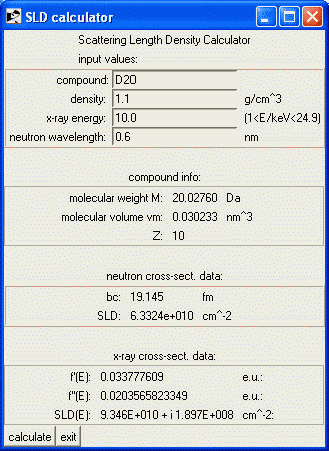
\includegraphics[width=0.329\textwidth,height=0.451\textwidth]{SLDcalculator.png}
\end{center}
\caption{Input menu for the scattering length density calculator}
\label{fig:SLDcalculator}
\end{figure}
The menu interface in Fig.\ \ref{fig:SLDcalculator} has for input
parameters, the sum formulae of the compound, its mass density in
g/cm$^3$, the x-ray energy in keV and the neutron wave length in nm.
In the compound name non-integer stoichiometry is supported, e.g.
H0.2O0.1 and H2O will calculate the same scattering length density.
However, the molecular volume $v_m$ and the molecular weight $M$ of
cause depend on such differences. The elements in the compound name
are case sensitive. Therefore you have to use \texttt{SiO2} instead
of \texttt{SIO2}. Also isotopes are handled like \texttt{C(13)}
(Carbon-13), \texttt{H(2)} (Deuterium), or \texttt{O(18)}
(Oxygen-18). For Deuterium next to \texttt{H(2)} also \texttt{D} can
be used.

Examples of how to format the compound name:
\begin{itemize}
\item Magnetite: \texttt{Fe3O4}, 5.15 g/cm$^3$
\item Eucryptite: \texttt{LiAlSiO4}, 2.67 g/cm$^3$
\item protonated toluene, \texttt{C7H8}, 0.865 g/cm$^3$
\item deuterated toluene, \texttt{C7D8} or \texttt{C7H(2)8}, 0.94 g/cm$^3$
\item mixture of 65/35 heavy water/light water, \texttt{(D2O)0.65(H2O)0.35}, 1.065 g/cm$^3$
\end{itemize}
From the compound name and the density first the molecular weight $M$, molecular volume $v_m$,
and total number of electrons $Z$ are calculated. Together with the tabulated neutron scattering length and
tabulated energy dependent scattering coefficient $f'(E)$ and $f''(E)$ the corresponding coherent
neutron scattering length $b_c=\sum_i b_i$, coherent neutron scattering length density
$\eta_{n,SLD}=b_c/v_m$  and
for x-rays the complex energy dependent scattering scattering length density
$\eta_{x,SLD}=\left(Z-(Z/82.5)^{2.37}+f'(E)+\imath f''(E)\right)/v_m$ of the compound are calculated.
